\section{Theorie}
\label{sec:Theorie}

\subsection{Entstehung von Röntgenstrahlung}

Fällt ein Elektron in ein Atom ein, kann es durch die Coulombkraft, zwischen dem positiven Kern
und dem Elektron, abgebremst werden. Dadurch sendet das Elektron ein Röntgenquant  aus, welches der
verlorenen Energie durch die Abbremsung entspricht. Das entstehende Spektrum ist kontinuierlich.
Bei vollständiger Abbremsung gilt für die minimale Wellenlänge:
\begin{equation}
  \lambda_{min} = \frac{h c}{e_0 U}
\end{equation}

Wenn Elektronen aus einer Glühkathode emittiert und auf eine Anode hin beschleunigt werden, ist zusätzlich
noch das charakteristische Spektrum zu sehen. Bei diesem Spektrum wird das Anodenmaterial so ionisiert, dass im Inneren
der Schale eine freie Stelle entsteht in die ein Elektron aus einer höheren Schale fallen kann. Dabei wird
ein Röntgenquant ausgesendet, welche die Differenz der beiden Energieniveaus besitzt.
\begin{equation}
  h \nu = E_m - E_n
\end{equation}

Das Spektrum besteht aus scharfen Linien, welche charakteristisch für das Material der Anode ist.
Innerhalb von Atomen mit mehreren Elektronen werden äußere Elektronen durch die Hüllenelektronen von
der Coulombkraft des Atomkerns abgeschirmt.
So gilt für die Bindungsenergie $E_n$ eines Elektrons auf der n-ten Schale:
\begin{equation}
  E_n = -R_{\infty} z_{eff}^2 \cdot \frac{1}{n^2}
\end{equation}

Dabei ist $R_{inf}$ die Rydberg-Energie, $z_{eff} = z - \sigma$ die effektive Kernladungszahl und $\sigma$ die Absorptionskonstante.

\subsection{Absorption von Röntgenstrahlung}
Bei der Absorption nimmt der Absorptionskoeffizient mit größer werdender Energie ab und steigt sprunghaft an, wenn
die Photonenenergie gerade größer ist als die Bindungsenergie der Elektronen aus der nächsten inneren Schale. Der
Comptoneffekt und der Photoeffekt sind bei der Absorption von Röntgenstrahlung unter $1$MeV die dominanten Prozesse.
Die Lage der Absorptionskanten $h \nu_{abs} = E_n - E_{\inf}$ ist nahezu identisch mit der Bindungsenergie.

\begin{figure}[H]
  \centering
  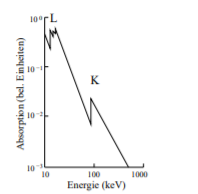
\includegraphics[height=5cm]{kante.PNG}
  \caption{Absorption in Abhängigkeit von der Energie \cite{sample}.}
  \label{fig:kathode}
\end{figure}

Mit der Berücktsichtigung der Feinstruktur gilt für die Bindungsenergie:
\begin{equation}
E_{n,j} = -R_{\infty} \left( z_{eff,1}^2 \cdot \frac{1}{n^2} + \alpha^2 z_{eff,2}^4 \cdot \frac{1}{n^3}
\left(\frac{1}{j+ \frac{1}{2}} - \frac{3}{4n} \right) \right)
\end{equation}

Wobei $\alpha$ die Sommerfeldsche Feinstrukturkonstante, $n$ die Hauptquantenzahl und $j$ der Gesamtdrehimpuls der
Elektronen ist.
Die Abschirmkonstante $\sigma_L$ kann mit der Energiedifferenz $E_L$ zweier L-Kanten bestimmt werden.
\begin{equation}
  \sigma_L = Z -\left(\frac{4}{\alpha} \sqrt{\frac{\Delta E_L}{R_{\infty}}} - \frac{5 \Delta E_L}{R_{\infty}} \right)^{1/2}
  \left(1 + \frac{19}{32} \alpha^2  \frac{\Delta E_L}{R_{\infty}} \right)^{1/2}
\end{equation}


Mithilfe der Bragg-Gleichung kann bei bekanntem Einfallswinkel $\Theta$ und Gitterkonstanten $d$, die gebeugte Wellenlänge
der Photonen bestimmt werden,
\begin{equation}
  2d \sin{\Theta} = n \lambda
\end{equation}

Dabei ist $n$ die Beugungsordnung.

Mit $E = \frac{hc}{\lambda}$ ergibt sich für die Winkelabhängigkeit der Energie
\begin{equation}
   E = \frac{hc}{2d \sin{\Theta}}
\end{equation}

\begin{figure}[H]
  \centering
  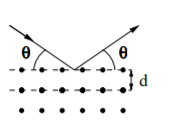
\includegraphics[height=5cm]{bragg.PNG}
  \caption{Bragg-Reflexion an einem Gitter \cite{sample}.}
  \label{fig:kathode}
\end{figure}
